\documentclass[11pt]{article}
% Language setting
% Replace `english' with e.g. `spanish' to change the document language
\usepackage[english]{babel}


% Set page size and margins
% Replace `letterpaper' with `a4paper' for UK/EU standard size
\usepackage[a4paper,top=3cm,bottom=3cm,left=2.2cm,right=2.2cm, marginparwidth=0.5cm]{geometry}

% Useful packages
\usepackage[utf8]{inputenc}

% Font setup with fontspec
\usepackage{fontspec}

\setmonofont{Fira Code}[Scale=0.9]

% Header setup (Format 2: Title with Section)
\usepackage{fancyhdr}
\pagestyle{fancy}
\fancyhead{}
\fancyhead[L]{M2 Deep Learning Coursework}
\fancyhead[R]{\rightmark}
\fancyfoot[C]{\thepage}
\renewcommand{\headrulewidth}{0.4pt}
\renewcommand{\sectionmark}[1]{\markright{#1}}

\usepackage{array}
\usepackage[most]{tcolorbox} % for inline code
\usepackage{amsmath}
\usepackage{graphicx}
\usepackage{caption}
\usepackage{subfigure} 
\usepackage[colorlinks=true, allcolors=blue]{hyperref}
\usepackage{authblk}
\usepackage{amssymb}
\usepackage{listings}
\usepackage{color}
\usepackage{xcolor}
\usepackage{float}
\usepackage{biblatex} %Imports biblatex package
\addbibresource{references.bib} %Import the bibliography file
\usepackage{wrapfig}
\usepackage{booktabs}
\usepackage{longtable}
\usepackage{pdflscape}

\usepackage[british]{datetime2}

\renewcommand{\floatpagefraction}{0.1}
\renewcommand{\textfraction}{0}

\definecolor{dkgreen}{rgb}{0,0.6,0}
\definecolor{gray}{rgb}{0.5,0.5,0.5}
\definecolor{mauve}{rgb}{0.58,0,0.82}
\definecolor{lightgray}{gray}{0.9}
\definecolor{softorange}{RGB}{254, 236, 220}
\definecolor{reddishbrown}{RGB}{183, 69, 25}

\lstdefinestyle{pythonstyle}{
  language=Python,
  frame=tb,
  aboveskip=3mm,
  belowskip=3mm,
  showstringspaces=false,
  columns=flexible,
  basicstyle={\ttfamily\small},
  numbers=left,
  numberstyle=\tiny\color{gray},
  keywordstyle=\color{blue},
  commentstyle=\color{green!50!black},
  stringstyle=\color{red!70!black},
  breaklines=true,
  breakatwhitespace=true,
  tabsize=4,
  captionpos=b,
  morekeywords={self, cls, __init__, None},
}

\lstdefinestyle{pseudocode}{frame=tb,
  language=Python,
  aboveskip=3mm,
  belowskip=3mm,
  showstringspaces=false,
  columns=flexible,
  basicstyle={\small\ttfamily},
  numbers=left,
  numberstyle=\tiny\color{gray},
  keywordstyle=\color{blue},
  commentstyle=\color{dkgreen},
  stringstyle=\color{mauve},
  breaklines=true,
  breakatwhitespace=true,
  tabsize=3
}

\lstdefinestyle{input}{frame=none,
  aboveskip=3mm,
  belowskip=3mm,
  showstringspaces=false,
  columns=flexible,
  basicstyle={\small\ttfamily},
  numbers=none,
  numberstyle=\tiny\color{gray},
  keywordstyle=\color{blue},
  commentstyle=\color{dkgreen},
  stringstyle=\color{mauve},
  breaklines=true,
  breakatwhitespace=true,
  tabsize=3,
  captionpos=b,
}


\definecolor{notebackground}{RGB}{250, 244, 237}
\definecolor{notetextgray}{RGB}{60, 60, 60}

\lstdefinestyle{notebookoutput}{
    backgroundcolor=\color{notebackground}, 
    basicstyle=\ttfamily\small\color{notetextgray}, 
    frame=none,                      
    xleftmargin=1.5em,               
    showstringspaces=false,
    numbers=none,                    
    breaklines=true,                 
    postbreak=\mbox{\textcolor{gray}{$\hookrightarrow$}\space},
}

% inline code display
\newtcbox{\inlinecode}{
  nobeforeafter, 
  colback=softorange,
  colframe=white,
  boxrule=0pt, 
  arc=1mm, 
  left=0pt, right=0pt, top=0pt, bottom=0pt,
  on line,
  fontupper=\scriptsize\ttfamily\color{reddishbrown}
}


% make title
\title{
\includegraphics[scale=0.2]{Cam_logo_bw.png}\\
\vspace{0.5cm}
M2 Deep Learning Coursework
}
\author{xl628}
\affil{Department of Physics}

\begin{document}

\maketitle

\vspace{1cm}
\noindent
\textbf{Document Statistics:} \\
Words in text: 2368 \\
Words in headers: 123 \\
Words outside text (captions, etc.): 477 \\

\section{Introduction}

Recent advances in large language models (LLMs) have opened up new possibilities for recasting time series prediction as a next-token prediction task. Inspired by insights from LLMTime\cite{gruver2024largelanguagemodelszeroshot}, we investigate the use of the \texttt{Qwen2.5-0.5B-Instruct} model\cite{qwen2025qwen25technicalreport} for forecasting tasks. We transform time series data into discrete tokens through appropriate preprocessing strategies. Furthermore, we employ Low-Rank Adaptation (LoRA)\cite{hu2021loralowrankadaptationlarge} to fine-tune the model, achieving significant improvements, all within tight computational constraints.

\section{Data and Preprocessing}

The methods presented here are implemented primarily in notebooks \texttt{00\_data\_exploration.ipynb} and \texttt{01\_llmtime\_preprocessing.ipynb}.

\subsection{LLMTIME Preprocessing Implementation}

Our dataset comprises synthetic time series generated by the Lotka-Volterra predator-prey model, structured as \inlinecode{(1000, 100, 2)}, indicating 1000 distinct simulations, each containing 100 temporal observations of two variables: predator and prey populations.

The paper \cite{gruver2024largelanguagemodelszeroshot} proposes a method to apply pretrained large language models (LLMs) for continuous time series prediction problems. It represents the time series as a string of numerical digits, and views time series forecasting as next-token prediction in text, unlocking the use of powerful pretrained models and probabilistic capacities, such as likelihood evaluation and sampling.

\paragraph{Scaling and Rounding}

The Qwen tokenizer inherently decomposes numeric strings into individual digit tokens. For instance, the string \inlinecode{"1.23"} is tokenized as \inlinecode{[16, 13, 17, 18]}, where \inlinecode{13} is the token ID of the decimal point.

To standardise the numeric range and control token length, we introduce a simple scaling factor $\alpha$:

$$x'_t=\frac{x_t}{\alpha}$$

where $\alpha$ is chosen based on the empirical data distribution.

Following scaling, we round the resulting values to a fixed number of decimal places to ensure consistency and reduce unnecessary precision. 

\begin{figure}[h!]
\centering
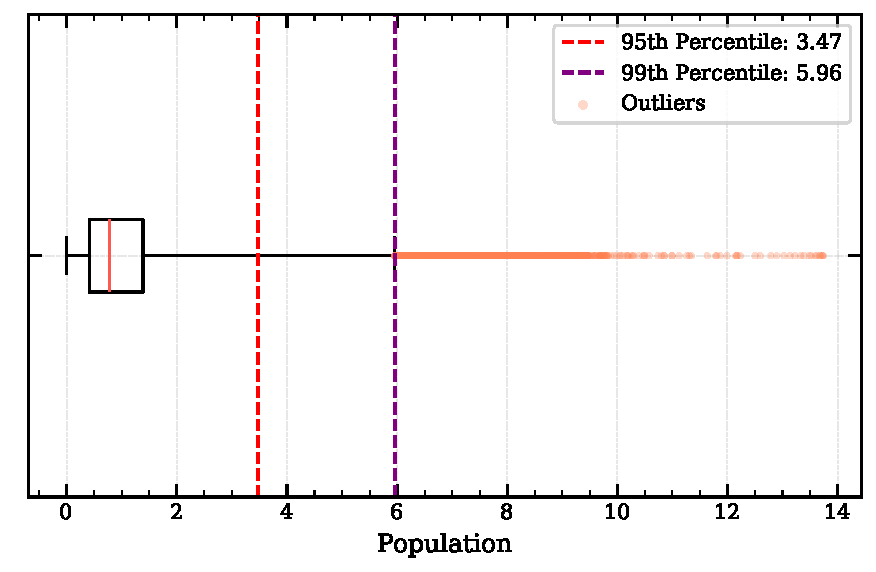
\includegraphics[width=0.47\textwidth]{./figures/boxplot.pdf}
\caption{Boxplot of unscaled population values from the entire dataset. The upper and lower edges of the box correspond to the 75th and 25th percentiles, respectively, while the red line in the box denotes the median. Most data falls within $[0, 2]$, and the 99th percentile is approximately 5.96. Coral-coloured points indicate outliers beyond the 99th percentile.}
\label{fig:box}
\end{figure}

\begin{figure}[h!]
\centering
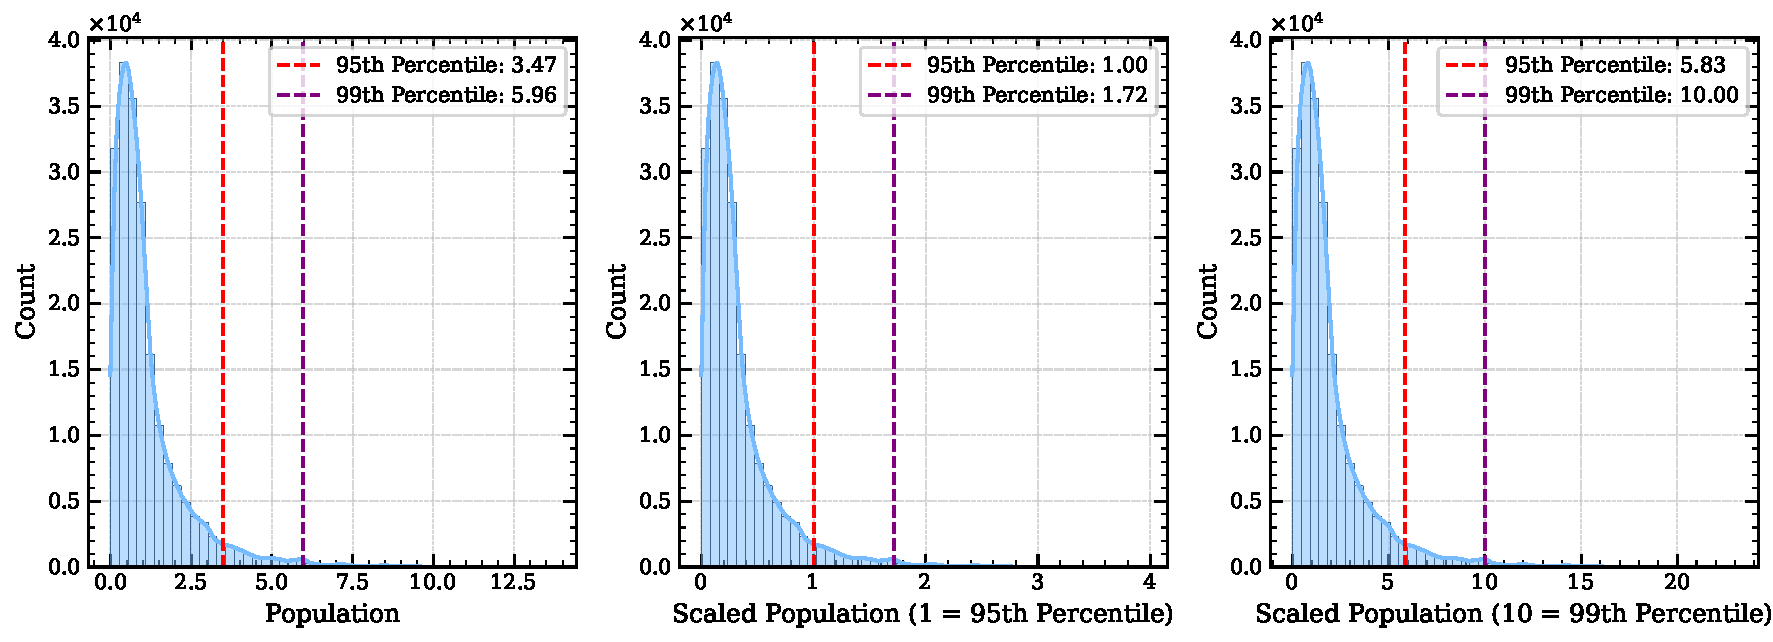
\includegraphics[width=0.99\textwidth]{./figures/dists.pdf}
\caption{From left to right: (i) unscaled population distribution, (ii) scaled with the 95th percentile mapped to 1, (iii) scaled with the 99th percentile mapped to 10. The 95th-percentile scaling results in most values being compressed into $[0, 1]$, thereby requiring greater decimal precision to retain information.}
\label{fig:dists}
\end{figure}

As seen in Figures~\ref{fig:box} and \ref{fig:dists}, the original data have been primarily distributed within the range $[0, 10]$, meaning the integer part typically consumes only one token. Further compression is therefore unnecessary and may result in information loss. In particular, Figure~\ref{fig:dist_95} illustrates how mapping the 95th percentile to 1 introduces noticeable roughness in the trajectories due to limited resolution in low-population regimes.

Although retaining more decimal places improves numeric precision, it incurs a higher token cost. For instance, maintaining three decimal places requires at least five tokens for every value (\inlinecode{"1.234"} $\rightarrow$ \inlinecode{[16, 13, 17, 18, 19]}).

To balance token efficiency and representational fidelity, we propose \textbf{scaling the 99th percentile to 10} and rounding to \textbf{two decimal places}. This transformation effectively preserves information while ensuring that roughly \textbf{99\% of values} require \textbf{only four tokens}. Figure~\ref{fig:dist_99} confirms that this strategy yields smoother and more faithful representations of population trajectories.


\begin{figure}[h!]
    \centering
    \subfigure[Scaling: 95th percentile $\rightarrow$ 1]{
        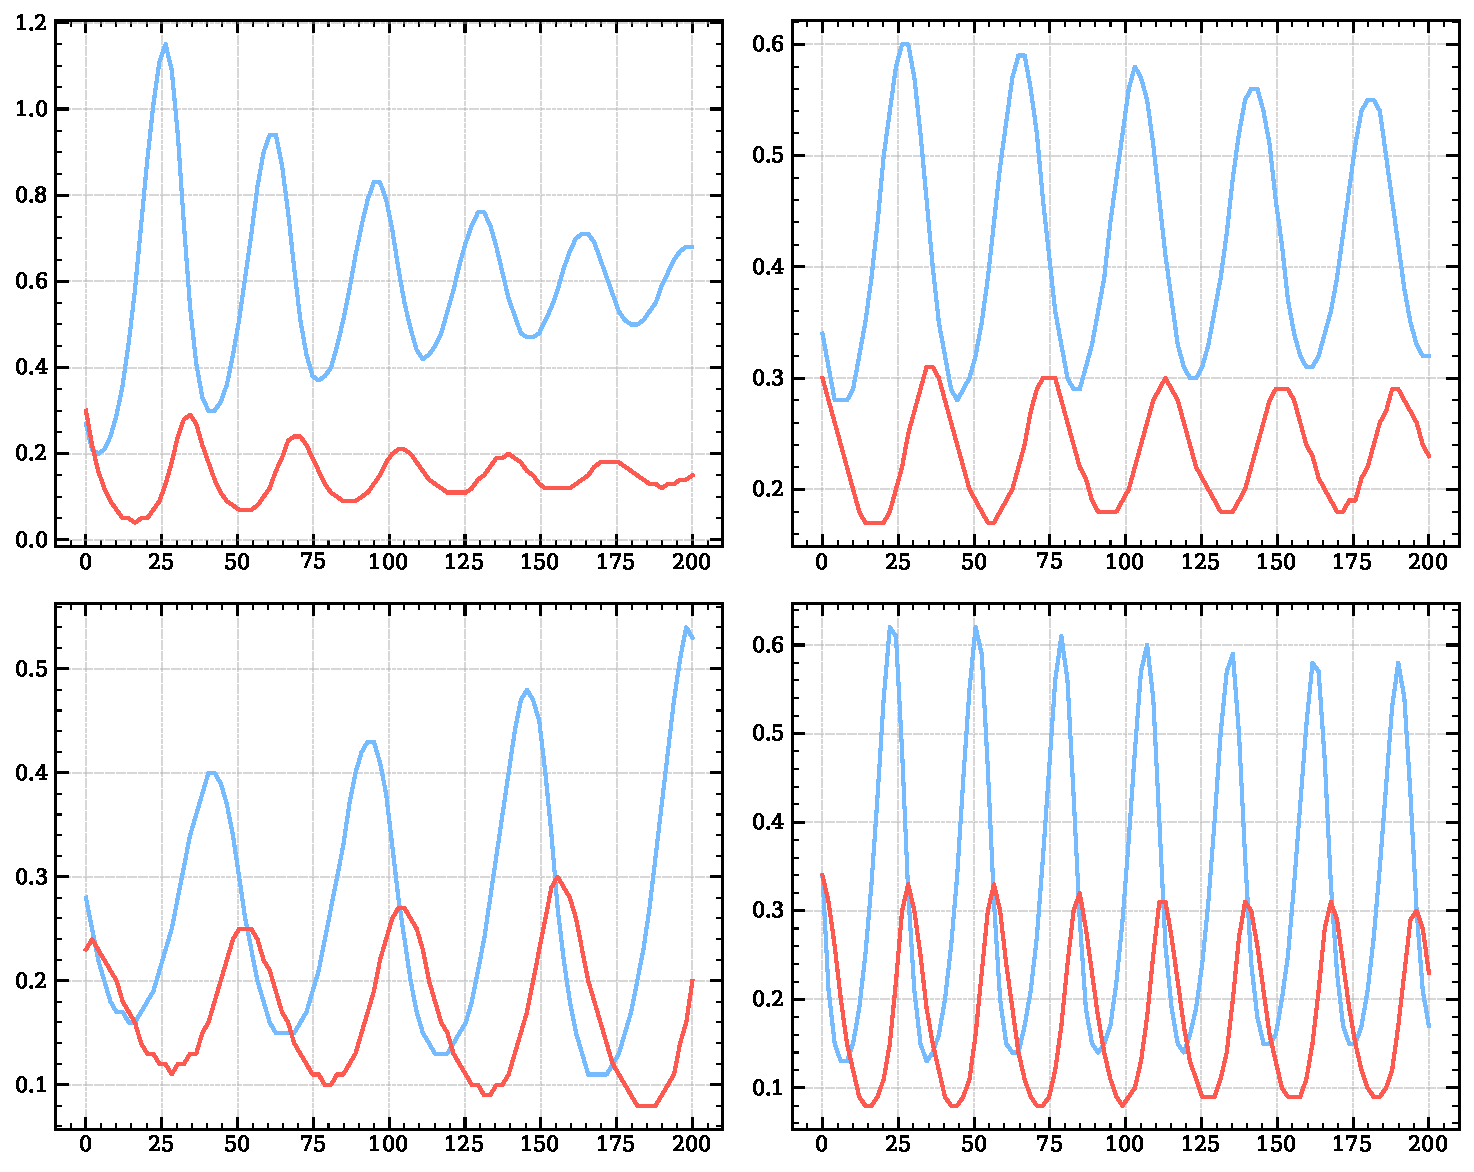
\includegraphics[width=0.47\textwidth]{./figures/traj_0.pdf}
        \label{fig:dist_95}
    }
    \hspace{0.01\textwidth}
    \subfigure[Scaling: 99th percentile $\rightarrow$ 10]{
        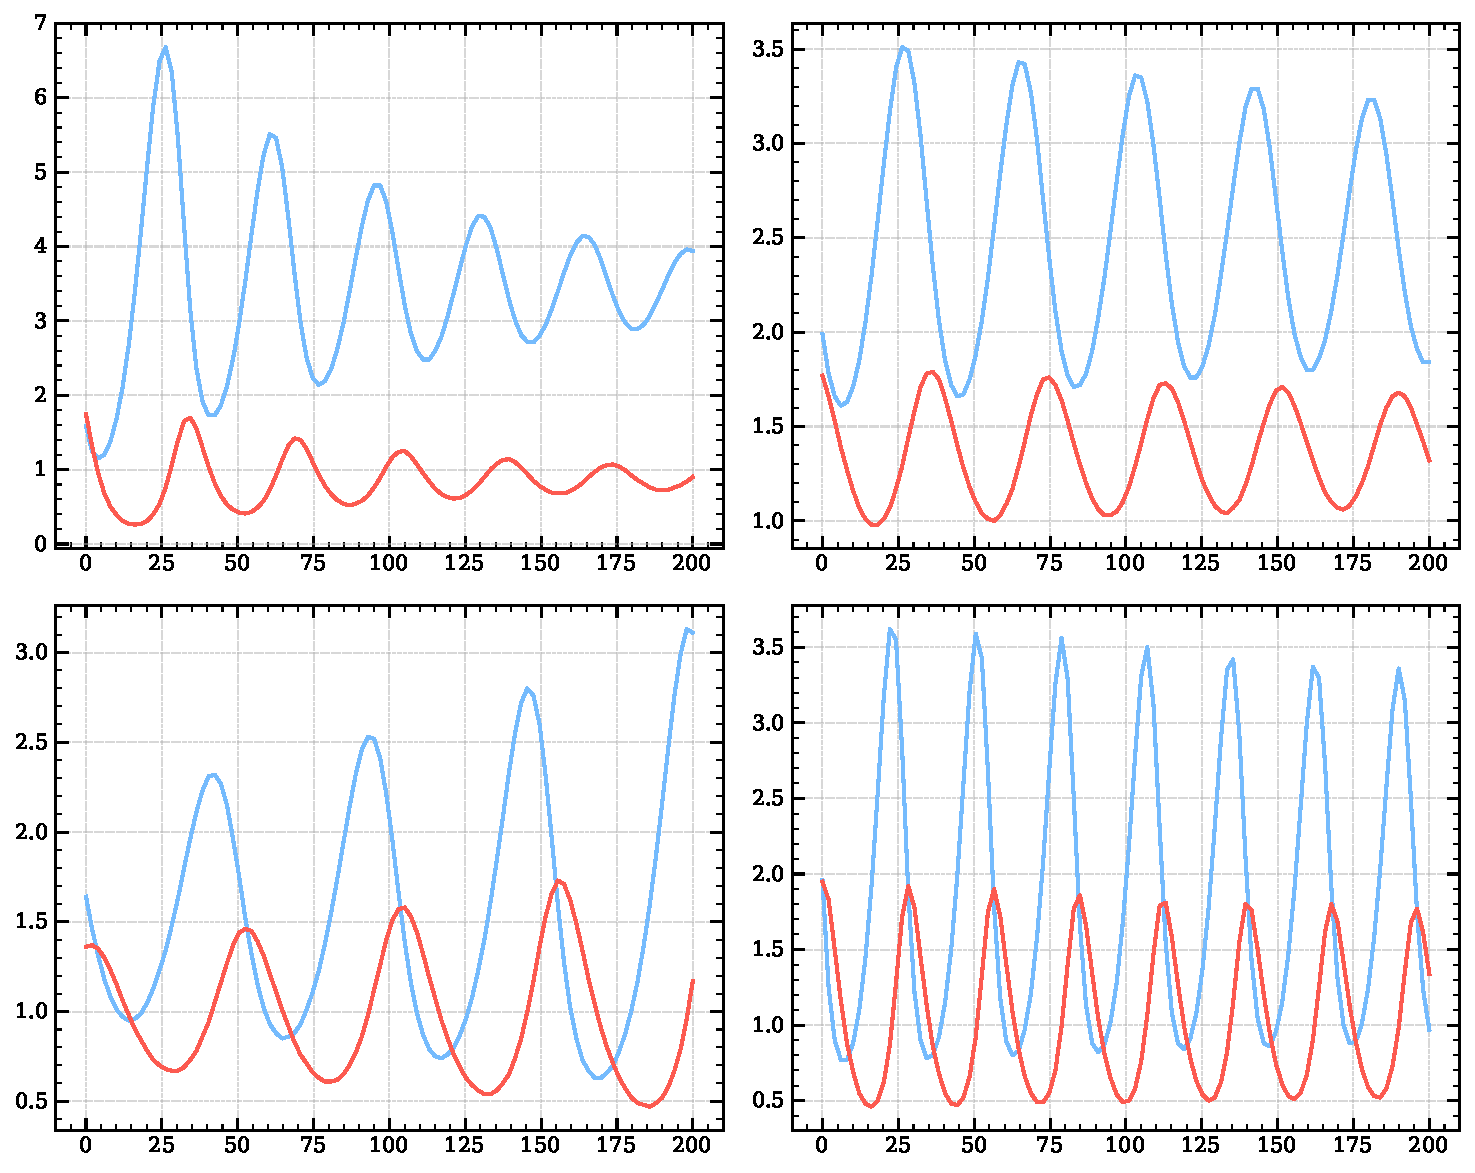
\includegraphics[width=0.47\textwidth]{./figures/traj_1.pdf}
        \label{fig:dist_99}
    }
    \caption{Effect of different scaling strategies on population trajectories across time points. In both cases, data were scaled based on the specified percentile of the dataset, then rounded to two decimal places. (a) shows visibly wiggly and rough behaviour in certain regions, likely due to information loss in low-population regimes. (b) exhibits smoother profiles, suggesting improved resolution preservation.}
    \label{fig:dist_scaling}
\end{figure}


\paragraph{Encoding Multivariate Data}

For encoding multivariate time series, we use the following convention:
\begin{itemize}
    \item Variables at the same timestep are separated by commas (\inlinecode{','}).
    \item Different timesteps are separated by semicolons (\inlinecode{';'}).

\end{itemize}
\subsection{Tokenization Example}

Let's walk through the process from raw data to tokenized sequences. Refer to Section 5 of the notebook \texttt{01\_llmtime\_preprocessing.ipynb}, where the full pipeline is demonstrated using our implemented preprocessor. An excerpt of the output is below:

\begin{lstlisting}[style=notebookoutput, caption={Examples showing the full processing pipeline applied to raw population trajectories (slices of 5 time steps). Each example includes the raw input, scaled and rounded version (using a scaling factor of 0.6007—corresponding to the 99th percentile of the training data—and two decimal places), the formatted string representation, and the corresponding tokenized sequence with integer token IDs.}]
--- Example 1 ---
Raw trajectory shape: (5, 2)
Raw trajectory:
[[0.94991744 1.040624  ]
 [0.74055135 0.7795419 ]
 [0.6822457  0.56439036]
 [0.7166742  0.40764433]
 [0.82451135 0.30028325]]

Scaled trajectory:
[[1.58 1.73]
 [1.23 1.3 ]
 [1.14 0.94]
 [1.19 0.68]
 [1.37 0.5 ]]

Formatted text:
1.58,1.73;1.23,1.30;1.14,0.94;1.19,0.68;1.37,0.50

Tokenized sequence (length 49):
[16, 13, 20, 23, 11, 16, 13, 22, 18, 26, 16, 13, 17, 18, 11, 16, 13, 18, 15, 26, 16, 13, 16, 19, 11, 15, 13, 24, 19, 26, 16, 13, 16, 24, 11, 15, 13, 21, 23, 26, 16, 13, 18, 22, 11, 15, 13, 20, 15]

...

--- Example 11 ---
Raw trajectory shape: (5, 2)
Raw trajectory:
[[0.96647114 1.094717  ]
 [0.75811523 0.94788396]
 [0.66393834 0.7895862 ]
 [0.6488795  0.6488567 ]
 [0.69528633 0.5355721 ]]

Scaled trajectory:
[[1.61 1.82]
 [1.26 1.58]
 [1.11 1.31]
 [1.08 1.08]
 [1.16 0.89]]

Formatted text:
1.61,1.82;1.26,1.58;1.11,1.31;1.08,1.08;1.16,0.89

Tokenized sequence (length 49):
[16, 13, 21, 16, 11, 16, 13, 23, 17, 26, 16, 13, 17, 21, 11, 16, 13, 20, 23, 26, 16, 13, 16, 16, 11, 16, 13, 18, 16, 26, 16, 13, 15, 23, 11, 16, 13, 15, 23, 26, 16, 13, 16, 21, 11, 15, 13, 23, 24]

\end{lstlisting}



\section{Baseline Evaluation}

In this section, we evaluate the forecasting capabilities of the untrained \texttt{Qwen2.5-0.5B-Instruct} model on a tokenized test set comprising 200 samples. The dataset was created via the notebook \texttt{01\_llmtime\_preprocessing.ipynb}.


\subsection{Untrained Qwen2.5-Instruct Performance}

Time series forecasting with pure time series methods typically prioritises recent data over distant past or future projections. Extending too far back can amplify the impact of non-stationarity, where older data ceases to represent current patterns due to shifts in the underlying process. Similarly, forecasting too far ahead compounds uncertainty, leading to larger prediction errors.

\begin{figure}[h!]
\centering
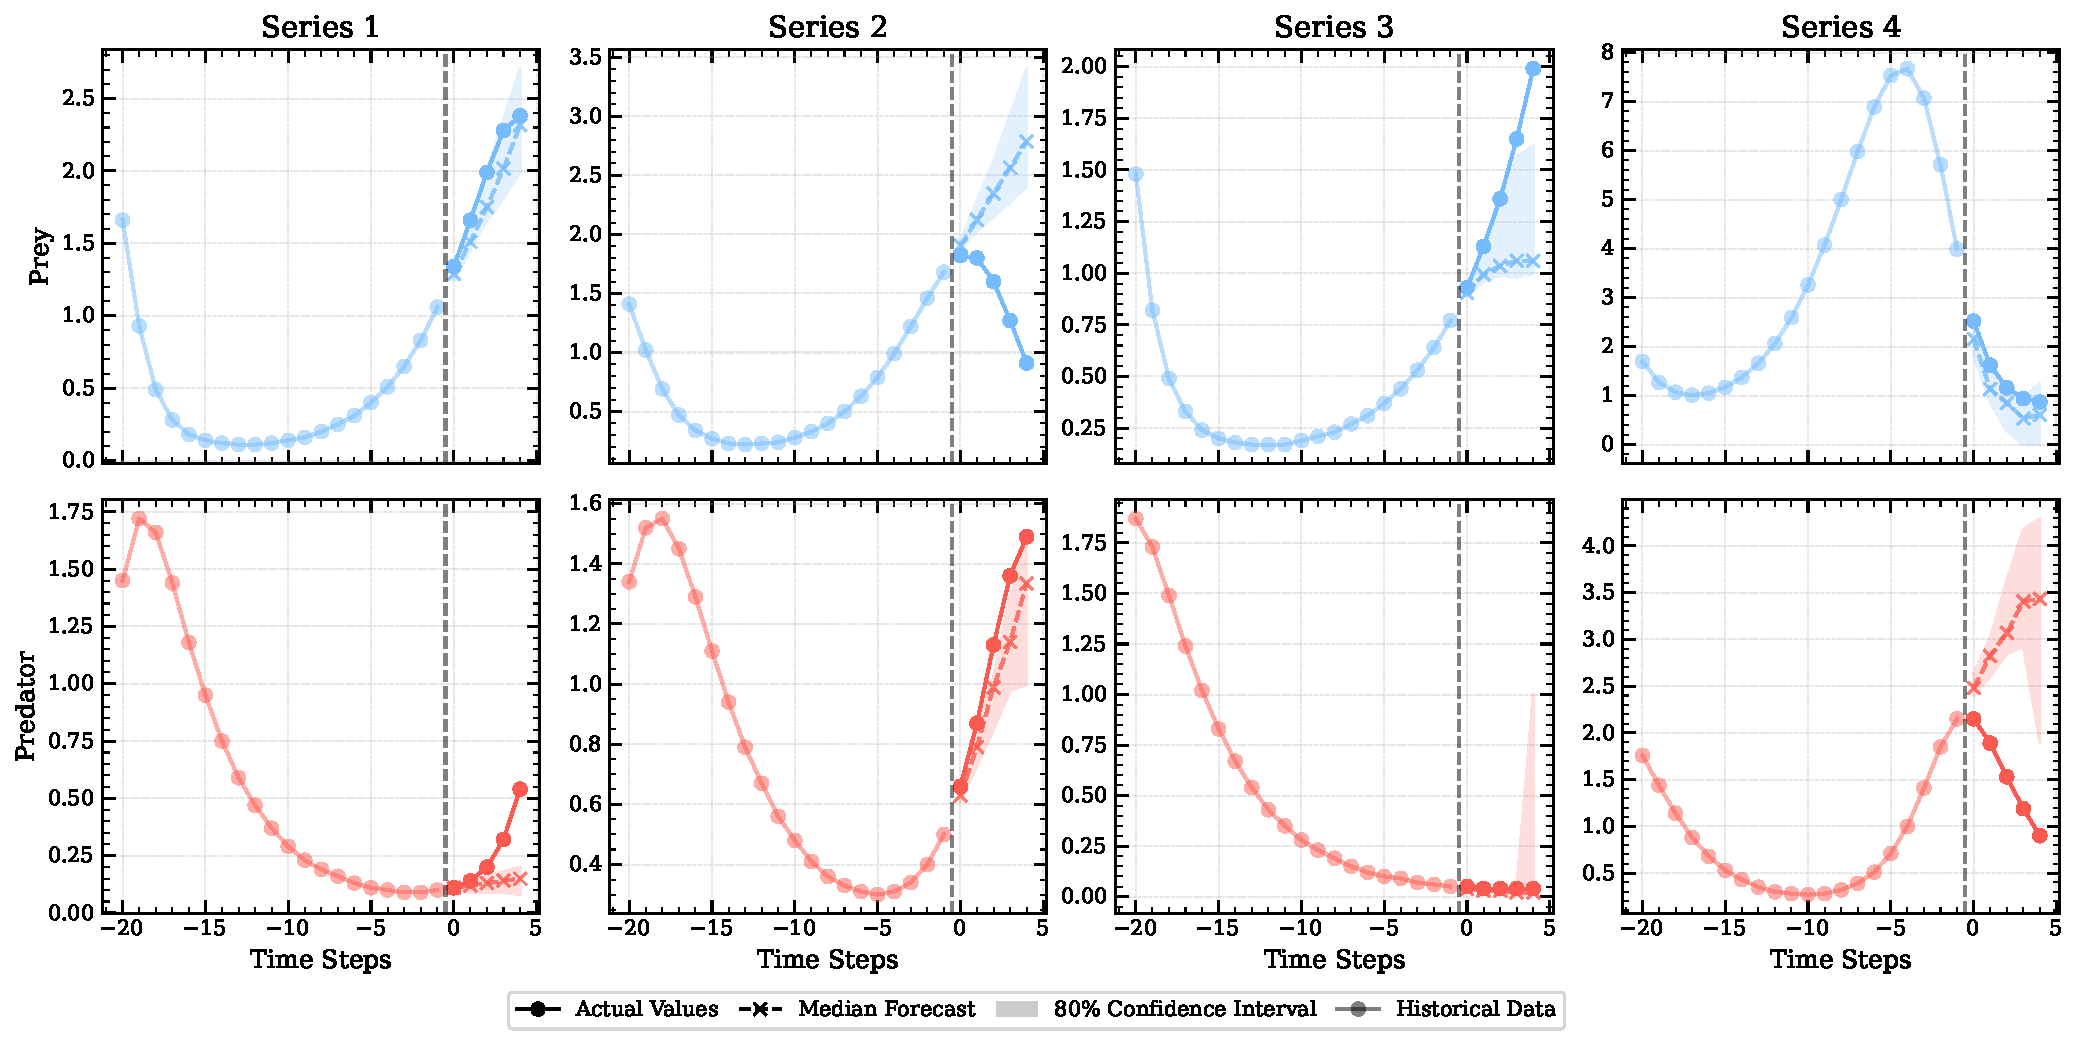
\includegraphics[width=0.99\textwidth]{./figures/baseline_pred.pdf}
\caption{Forecasts generated by the \textbf{untrained} \texttt{Qwen2.5-0.5B-Instruct} model on four test samples. Cross markers denote point predictions, while shaded regions represent estimated 80\% confidence intervals from Monte Carlo sampling (context steps = 20, forecast steps = 5, temperature = 0.7, top-k = 20).}
\label{fig:baseline}
\end{figure}


Given these constraints, we employ relatively short context (20 steps) and forecast lengths (5 steps) in our evaluation. We utilise Monte Carlo sampling, generating 20 samples per forecast from the model's probabilistic distribution, allowing us to estimate an approximate 80\% confidence interval. Figure \ref{fig:baseline} illustrates four forecasts produced by the untrained model.



Since the model lacks specific training for this task, it frequently produces non-numeric or malformed outputs. We address these issues post hoc, primarily by imputing the last observed valid value in cases of such invalid outputs.


We evaluate the model’s predictions using standard metrics, presented in Table \ref{tab:model_comparison}, with comparisons to a naive baseline that repeats the last observed value for each variable.




The results demonstrates that the untrained \texttt{Qwen2.5-0.5B-Instruct} model consistently outperforms the naive baseline across all the metrics. This suggests that, despite the absence of explicit task-specific training, the model captures some underlying structure from tokenized numeric sequences, benefiting from its pretrained knowledge. 

Additionally, effective uncertainty quantification is critical for assessing forecast reliability, especially in financial contexts where risk management heavily relies on understanding predictive uncertainty. 

We measure uncertainty quantification through the empirical coverage metric, which measures the proportion of true values falling within the model’s 80\% confidence intervals, derived from Monte Carlo sampling. Ideally, this should be close to 0.8 (80\%). However, our untrained model's coverage (0.3325) is notably lower than desired, suggesting the generated confidence intervals are too narrow or misaligned with the true data distribution. 

Adjusting sampling parameters such as temperature or top-k/top-p might mitigate overly deterministic predictions, yet improvements to the model’s core forecasting capability through fine-tuning would likely yield greater overall reliability improvements.

\section{LoRA Fine-tuning}

In this section, we employ Low-Rank Adaptation (LoRA)\cite{hu2021loralowrankadaptationlarge} to fine-tune the \texttt{Qwen2.5-0.5B-Instruct} model specifically for our time series forecasting task.

LoRA inserts trainable low-rank adapters into existing weights without modifying the original parameters. Each LoRA-adapted module performs:
\begin{equation}
Y = XW_0 + X\Delta W = XW_0 + XAB\cdot\frac{\alpha}{r}
\end{equation}
where $A \in \mathbb{R}^{r \times \text{in\_dim}}$ and $B \in \mathbb{R}^{\text{out\_dim} \times r}$ are low-rank matrices with rank $r \ll min(\text{in\_dim}, \text{out\_dim})$. Here, $r$ controls the rank of the adaptation, and $\alpha$ is a scaling factor set equal to $r$ in our implementation.

LoRA factorizes the parameter update $\Delta W \in \mathbb{R}^{\text{out\_dim} \times \text{in\_dim}}$ into two smaller matrices ($A$, $B$), significantly reducing the number of trainable parameters from $\text{in\_dim} \times \text{out\_dim}$ to $r \times (\text{in\_dim} + \text{out\_dim})$.

In our implementation, LoRA is specifically applied to the query and value projection matrices (\inlinecode{q\_proj}, \inlinecode{v\_proj}) within each transformer layer's self-attention mechanism. Additionally, we leave the final layer's bias parameters unfrozen to bias the model towards numerical tokens in our dataset.



See tnotebook \texttt{04\_lora\_implementation.ipynb} for detailed implementation and a tentative preliminary training result.

\begin{table}[h!]
\centering
\caption{Hyperparameter settings for initial LoRA fine-tuning of \textbf{Qwen2.5-0.5B-Instruct}. Context length represents the maximum token sequence processed, while stride indicates the sliding window step size for processing overlapping data segments.}
\begin{tabular}{ll}
\toprule
\textbf{Hyperparameter} & \textbf{Values} \\
\midrule
\multicolumn{2}{c}{\textit{Training Parameters}} \\
\midrule
Batch Size & 8 \\
Maximum Steps & 1000 \\
Learning Rate & $1 \times 10^{-5}$ \\
Evaluation Steps & 50 \\
Optimizer & AdamW \\
\midrule
\multicolumn{2}{c}{\textit{LoRA Configuration}} \\
\midrule
LoRA Rank ($r$) & 4 \\
LoRA $\alpha$ & 4 (same as rank) \\
Target Modules & ["q\_proj", "v\_proj"] \\
\midrule
\multicolumn{2}{c}{\textit{Data Parameters}} \\
\midrule
Context Length & 512 \\
Stride & 256 \\
\bottomrule
\end{tabular}
\label{tab:hyperparameters}
\end{table}


\subsection{Initial Experiment}

We initially train the 0.5B parameter model with LoRA configurations based on the default hyperparameters in Table \ref{tab:hyperparameters} on an NVIDIA A100 GPU (40GB).


\begin{figure}[h!]
\centering
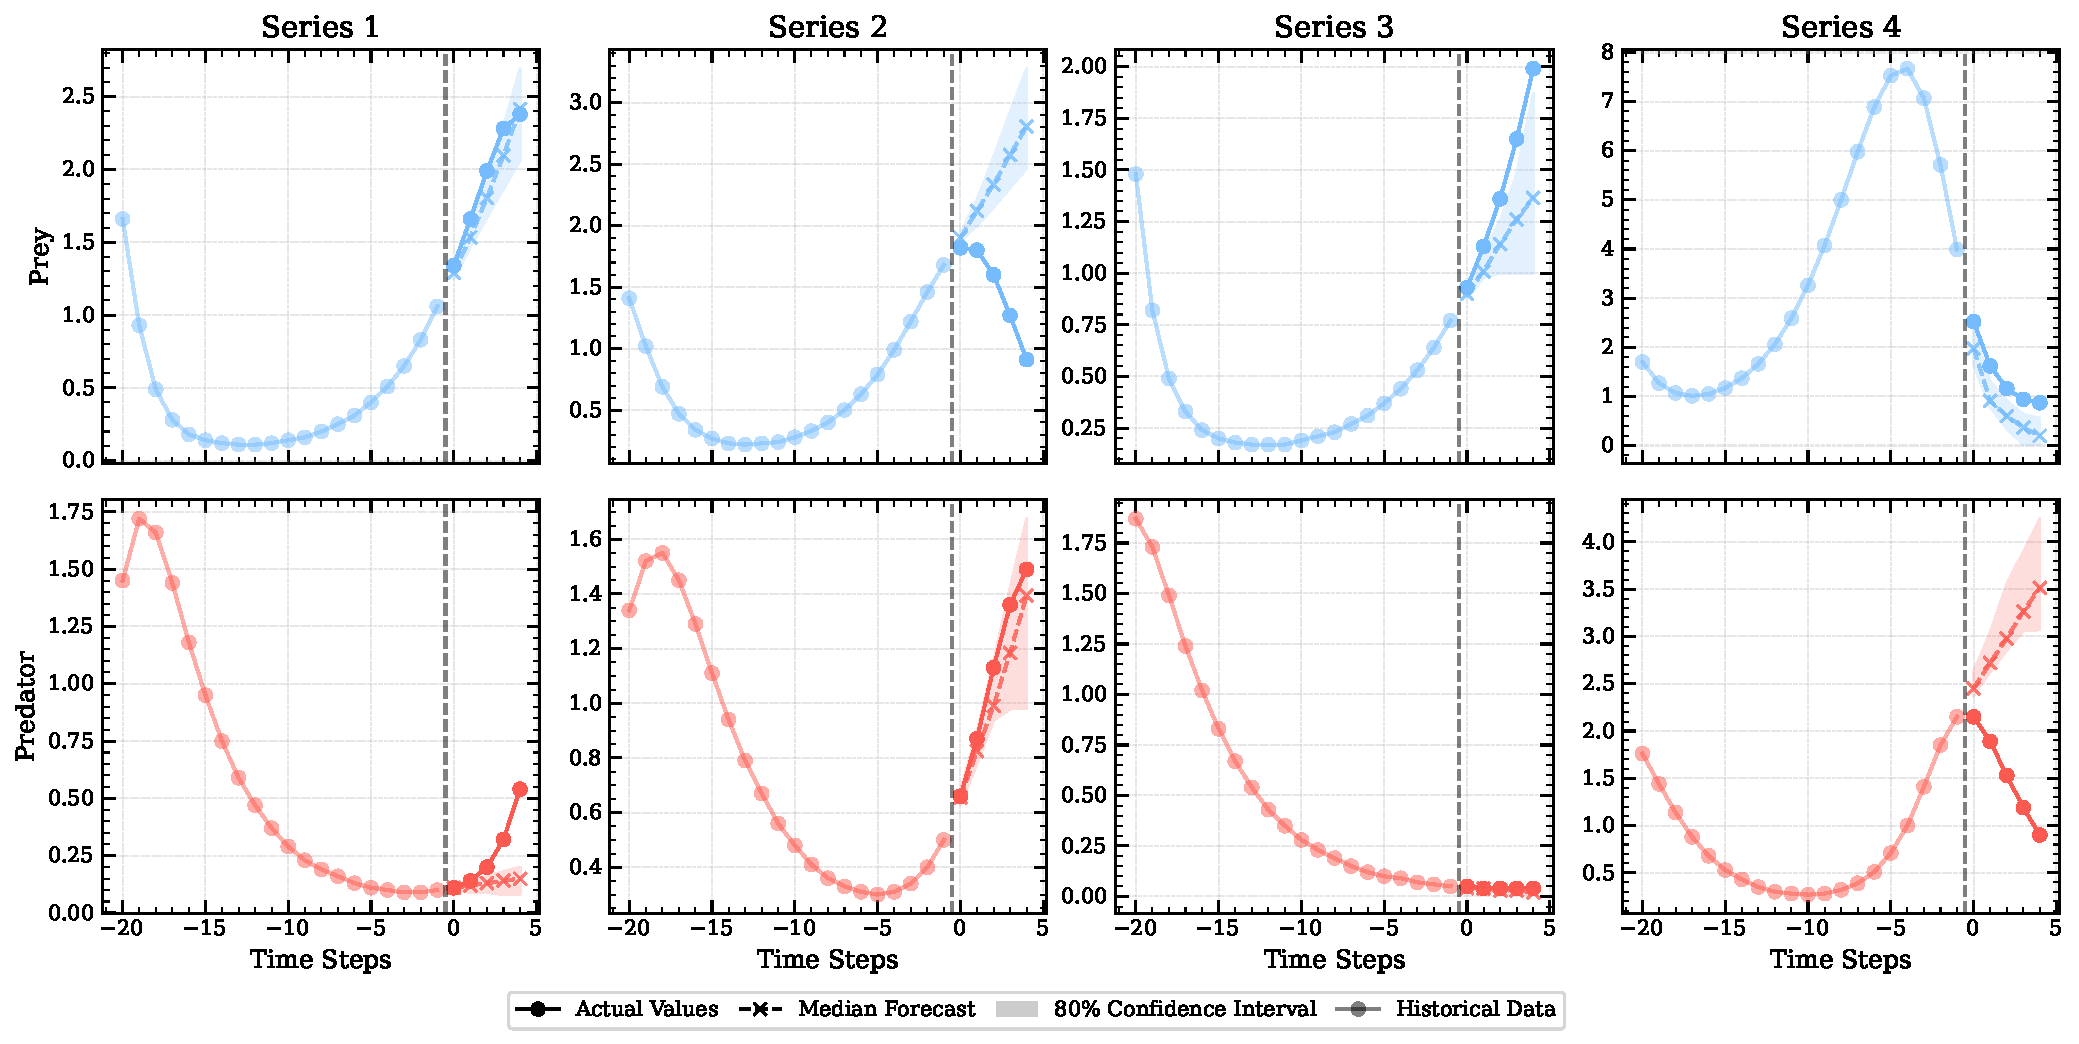
\includegraphics[width=0.99\textwidth]{./figures/initial_pred.pdf}
\caption{Forecasts produced by the \textbf{initial LoRA fine-tuning} \texttt{Qwen2.5-0.5B-Instruct} model on four test samples. Same context and forecast length and sampling parameters as in Figure \ref{fig:baseline}.}
\label{fig:intial_pred}
\end{figure}

Training and evaluation loss curves (cross-entropy) are presented in Figure \ref{fig:initial_loss}. Both training and evaluation losses steadily decrease, indicating effective learning without noticeable overfitting.


After 1000 steps training with LoRA fine-tuning, the model consistently improves all error metrics, presented in Table \ref{tab:model_comparison}. These improvements demonstrate that LoRA gradually adapts the model to better fit our forecasting task.

The small increase in coverage and decrease in interval width is also a step forward, showing that LoRA enhances the model’s ability to quantify uncertainty.

These improvements are meaningful but not dramatic. However, they suggest that further training and fine-tuning—such as hyperparameter search—could yield better outcomes. This will be the focus of our next steps.


\begin{table}[h!]
\centering
\caption{Model Performance Comparison}
\begin{tabular}{lcccc}
\hline
\textbf{Metric} & \textbf{Naive Predict} & \textbf{Untrained Baseline} & \textbf{Initial LoRA} & \textbf{Final LoRA} \\
\hline
MSE            & 1.4202     & 0.8832     & 0.8069     & 0.0579     \\
RMSE           & 0.8451     & 0.6217     & 0.5903     & 0.1289     \\
MAE            & 0.7612     & 0.5244     & 0.4947     & 0.1049     \\
MAPE (\%)      & 55.73      & 36.23      & 34.90      & 6.53       \\
SMAPE (\%)     & 42.69      & 31.62      & 29.18      & 6.20       \\
Coverage       & --         & 0.3325     & 0.3520     & 0.5680     \\
Interval Width & --         & 0.5100     & 0.5050     & 0.1661     \\
\hline
\end{tabular}
\label{tab:model_comparison}
\end{table}


\begin{figure}[h!]
\centering
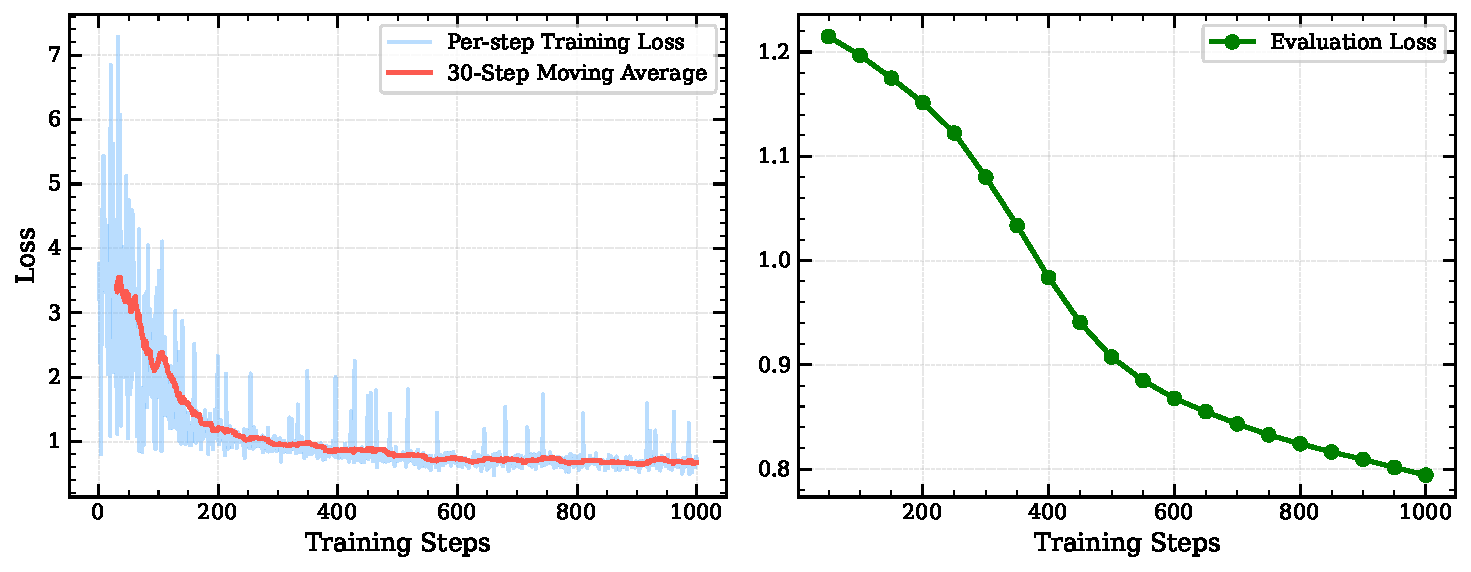
\includegraphics[width=0.9\textwidth]{./figures/training_0.pdf}
\caption{Initial training loss curves. 
Left: Per-step training loss (light blue) with a 30-step moving average (red) shows a consistent downward trend. 
Right: Evaluation loss (green) also steadily declines. }
\label{fig:initial_loss}
\end{figure}

\begin{figure}[h!]
\centering
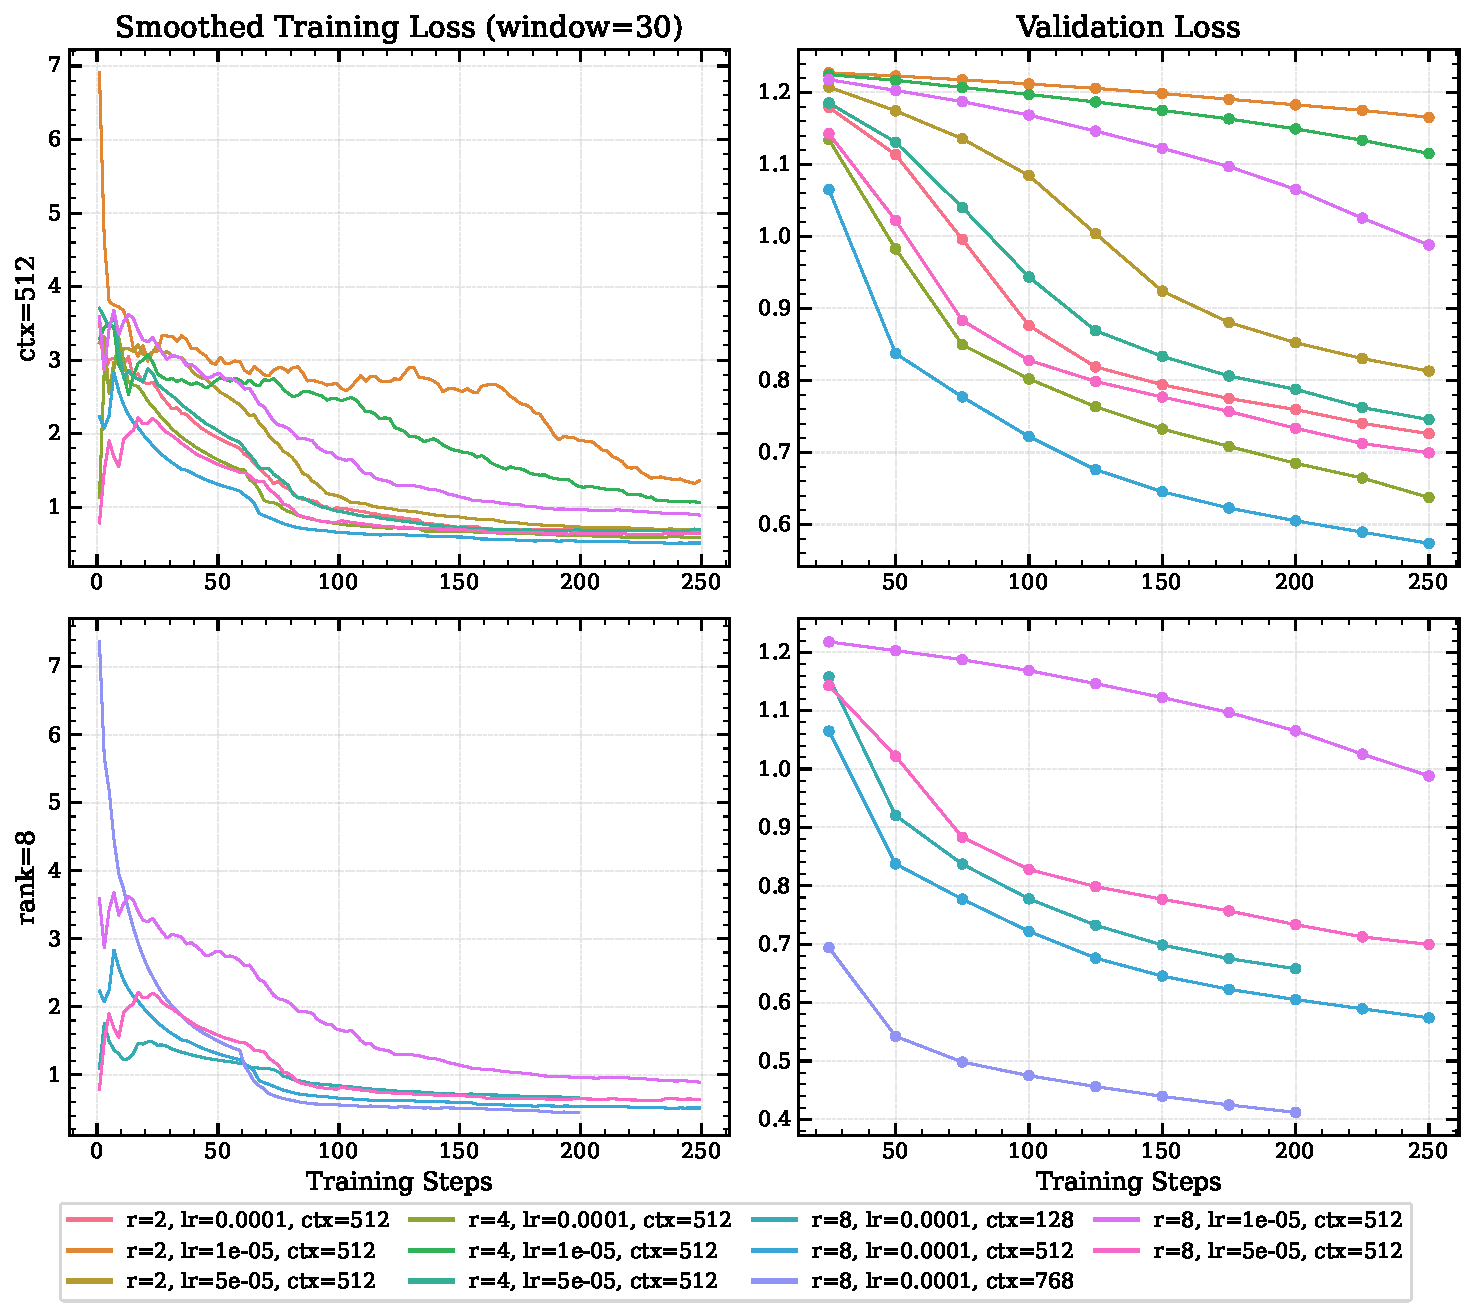
\includegraphics[width=0.9\textwidth]{./figures/hyperparameter_comparison_subplots.pdf}
\caption{Comparison of smoothed training loss (left column) and validation loss (right column) across different LoRA ranks, learning rates, and context lengths. 
Top row: Results for context length 512 across multiple ranks ($r=2, 4, 8$) and learning rates ($1\text{e-}5$, $5\text{e-}5$, $1\text{e-}4$). 
Bottom row: Fixed the best parameters from the previous search — rank $r=8$ and learning rate $\text{lr}=0.0001$ — and varied context lengths (128, 512, 768), while also including the other two learning rates at context length 512 for comparison.}
\label{fig:hyperparameter_comparison_subplots}
\end{figure}


\subsection{Hyperparameter Tuning}

\begin{table}[h!]
\centering
\caption{Hyperparameter configurations used for LoRA fine-tuning of Qwen2.5-Instruct. }
\begin{tabular}{ll}
\toprule
\textbf{Hyperparameter} & \textbf{Values} \\
\midrule
\multicolumn{2}{c}{\textit{Hyperparameters Varied During Search}} \\
\midrule
Learning Rate & $\{1 \times 10^{-5}, 5 \times 10^{-5}, 1 \times 10^{-4}\}$ \\
LoRA Rank ($r$) & $\{2, 4, 8\}$ \\
Context Length & $\{128, 512, 768\}$ \\
\midrule
\multicolumn{2}{c}{\textit{Fixed Hyperparameters}} \\
\midrule
Batch Size & 8 \\
Maximum Steps (Main) & 250 \\
Maximum Steps (Context) & 200 \\
Evaluation Frequency & 25 \\
Optimizer & AdamW \\
LoRA $\alpha$ & Same as rank \\
Target Modules & ["q\_proj", "v\_proj"] \\
Stride & 256 \\
\bottomrule
\end{tabular}
\label{tab:search_configs}
\end{table}

\begin{figure}[h!]
\centering
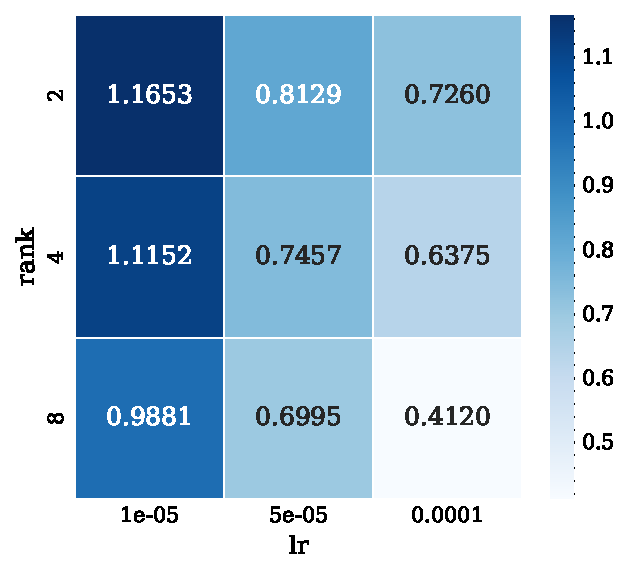
\includegraphics[width=0.4\textwidth]{./figures/best_loss_heatmap.pdf}
\caption{Heatmap of best validation loss across different combinations of LoRA rank and learning rate (lr). Lighter shades of blue indicate lower loss values, reflecting better model performance.}
\label{fig:best_loss_heatmap}
\end{figure}

We performed hyperparameter tuning through grid search, adjusting learning rates, LoRA ranks, and context lengths according to configurations shown in Table \ref{tab:search_configs}. The tuning process consisted of two stages: an initial exploration of learning rates and LoRA ranks, followed by context length optimisation based on the best-performing parameters identified initially.

\newpage
The training and validation losses of all parameter combinations are showed in Figure \ref{fig:hyperparameter_comparison_subplots}, showing \textbf{higher LoRA ranks}, \textbf{larger learning rates}, and \textbf{longer context lengths} yield faster convergence and improved model performance. 

Figure \ref{fig:best_loss_heatmap} summarises the optimal validation loss across different combinations of LoRA rank and learning rate. Again, the trend shows that increasing both the LoRA rank and the learning rate leads to improved model performance, as evidenced by decreasing validation loss.



The results indicate that the best configuration in this search is \inlinecode{learning\_rate=1e-4}, \inlinecode{lora\_rank=8}. We further explored context lengths of \inlinecode{[128, 512, 768]}, finding that the longest context length \inlinecode{ctx\_length=768} yielded the best performance. Thus, these hyperparameters were selected for the final training phase.

\newpage
\subsection{Final Model Training}

To manage the FLOPS budget, we limited the final training to 2,000 steps, although training curves suggest that additional training may yield further improvements.

An important observation from this final training is the absence of previously encountered non-numeric or unstructured outputs, as evidenced by the logging files. This indicates that the model has effectively learned the structure of the numeric time series tokens. In other words, the fine-tuned model demonstrates strong task-specific adaptation.

The final LoRA model achieves extraordinary improvements in all evaluated metrics compared to prior models, as detailed in Table \ref{tab:model_comparison}. For instance, the mean absolute error (MAE) dramatically drops from 0.7612 (naive), 0.5244 (untrained) and 0.4947 (initial LoRA) down to 0.1049 (final LoRA).

\begin{figure}[h!]
\centering
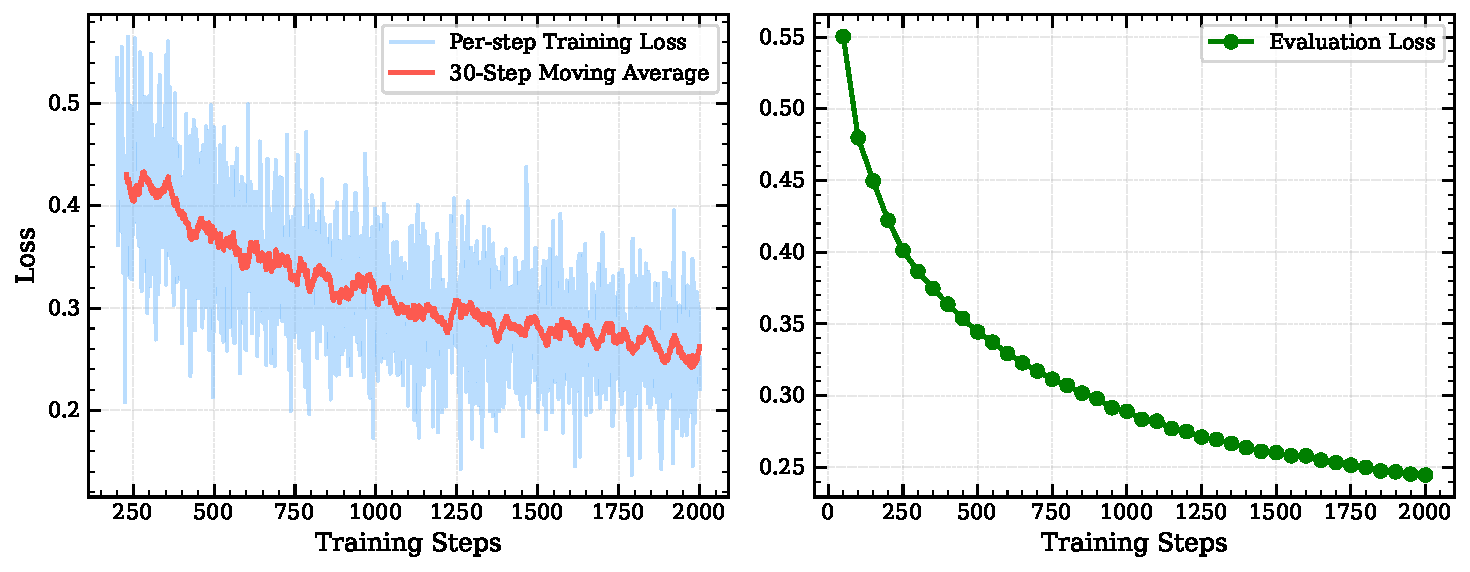
\includegraphics[width=0.9\textwidth]{./figures/training_final.pdf}
\caption{Final training of the best-performing model. 
Left: Per-step training loss with a 30-step moving average, shown from step 200 onward, continues to decrease. 
Right: Evaluation loss maintains a consistent downward trajectory.}
\label{fig:training_final}
\end{figure}

Coverage increases to 0.5680, a significant leap from 0.3325 (untrained) and 0.3520 (initial LoRA), with a much narrower interval width (0.1661 vs. 0.5100 and 0.5050). This combination indicates that the final LoRA model not only predicts more accurately but also provides tighter, better-calibrated confidence intervals. However, since coverage remains below the desired 0.8, there is room for additional refinement in uncertainty quantification.

Although performance substantially improved, the continual downward trends observed in both training and evaluation losses (Figure \ref{fig:training_final}) suggest the potential for even greater performance with extended training. The incomplete hyperparameter search also implies that the model may not yet be at its peak performance.

\begin{figure}[h!]
\centering
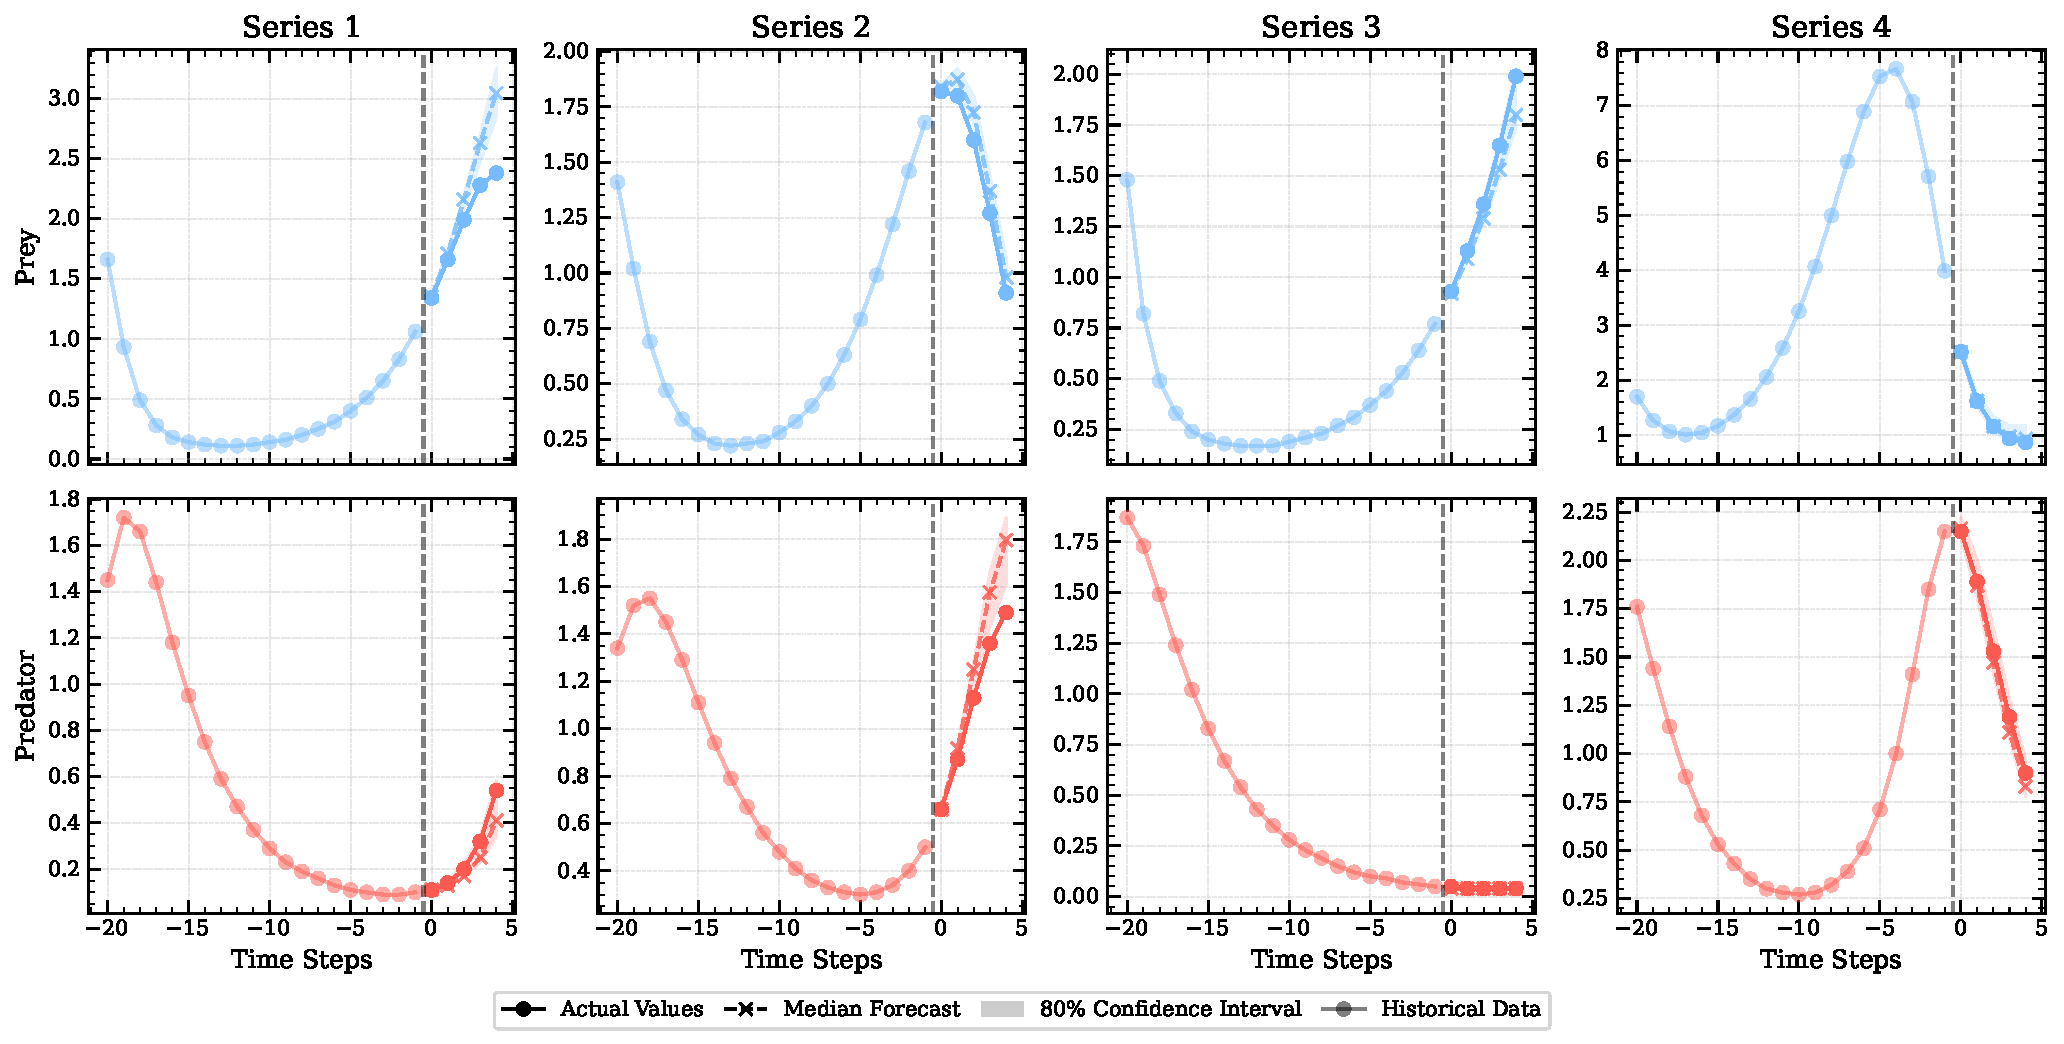
\includegraphics[width=0.9\textwidth]{./figures/final_pred.pdf}
\caption{Forecasts generated by the \textbf{Final LoRA fine-tuned} \texttt{Qwen2.5-0.5B-Instruct} model on four test samples, using the same context, forecast length, and sampling parameters as Figure \ref{fig:baseline}. The prediction trajectories show significant improvement over those in Figures \ref{fig:intial_pred} and \ref{fig:baseline}.}
\label{fig:final_pred}
\end{figure}

Forecast visualizations in Figure \ref{fig:final_pred} illustrate clear improvements compared to earlier model versions (Figures \ref{fig:intial_pred} and \ref{fig:baseline}), reinforcing the significant advancements achieved through the final LoRA fine-tuning.





\section{FLOPS Calculation for Qwen2.5-Instruct Models}

The notebook \texttt{03\_flops\_calculation.ipynb} provides examples of FLOPs calculation specified to Qwen2.5-0.5B hyperparameters. A concise yet comprehensive summary of the computational breakdown is presented in Table \ref{tab:transformer-computation}.

\subsection*{Notation \& FLOPS Accounting Table}

\begin{table}[h!]
\centering
\renewcommand{\arraystretch}{1.2}
\begin{tabular}{ll}
\toprule
\textbf{Symbol} & \textbf{Description} \\
\midrule
$B$ & Batch size (number of sequences per forward pass) \\
$S$ & Sequence length (number of tokens per sequence) \\
$H$ & Hidden size (embedding dimension) \\
$I$ & Intermediate size in the MLP block \\
$V$ & Vocabulary size for the language modeling head \\
$L$ & Number of transformer layers in the model \\
$N_h$ & Number of attention heads \\
$D_h$ & Dimension per head ($D_h = H / N_h$) \\
$r$ & LoRA rank (dimensionality of low-rank adapters) \\
$M$ & Number of LoRA-injected modules (e.g., $2L$ for Q and V projections) \\
$T$ & Number of training steps or optimization iterations \\
$\mathcal{F}_{\cdot}$ & FLOPs (floating-point operations) for a given module or total \\
\bottomrule
\end{tabular}
\caption{Notation used in FLOPs and LoRA computation.}
\label{tab:flops-notation}
\end{table}

In this analysis, we account for basic operations as in Table \ref{tab:flops_primitives}.

\begin{table}[h!]
    \centering
    \begin{tabular}{|l|c|}
        \hline
        \textbf{Operation} & \textbf{FLOPS} \\
        \hline
        Addition/Subtraction/Negation (float or integer) & 1 \\
        Multiplication/Division/Inverse (float or integer) & 1 \\
        ReLU/Absolute Value & 1 \\
        Exponentiation/Logarithm & 10 \\
        Sine/Cosine/Square Root & 10 \\
        \hline
    \end{tabular}
    \caption{FLOPS accounting for primitive operations.}
    \label{tab:flops_primitives}
\end{table}

Matrix multiplication \( m \times n \) by \( n \times p \) (without bias) is \( m \times p \times (2n - 1) \) FLOPS (\( n \) multiplications, \( n-1 \) additions per element). With bias, it’s \( m \times p \times 2n \) (adds \( n \) additions for bias).

This represents a simplified accounting method. Other primitives that cannot be expressed with these are assumed to be 0 FLOPS, such as array indexing, memory management, etc.



\subsection{Detailed FLOPS Analysis}



\subsubsection{Input Processing}

\paragraph{Token Embeddings}
After tokenization, each input token is mapped to an $H$-dimensional vector via an embedding lookup. Conceptually, this corresponds to a matrix multiplication of shape $B \times S \times V @ V \times H$ requiring $B \times S \times H \times (2V-1)$ FLOPS. However, in practice, this operation is implemented as a lookup table and conventionally considered to require \textbf{zero FLOPS}.

\paragraph{Positional Encodings} 
Qwen2.5 employs \textbf{Rotary Position Embeddings (RoPE)}~\cite{su2023roformerenhancedtransformerrotary} to encode positional information within the attention mechanism through structured rotations of query and key vectors.

For simplicity, we approximate this by assuming the addition of precomputed positional encodings to token embeddings. With embeddings of shape $B\times S \times H$ and positional encodings of shape $S \times H$ (broadcasted across the batch dimension), this requires $B \times S \times H$ FLOPS for element-wise addition.


\subsubsection{Transformer Layers}

Each of the $L$ identical transformer layers processes the sequence as follows:

\paragraph{Root Mean Square Layer Normalization (RMSNorm)}
Qwen2.5 applies RMSNorm~\cite{zhang2019rootmeansquarelayer} to the input tensor $X \in \mathbb{R}^{B \times S \times H}$ according to:
\[
\tilde{x}_i = \frac{x_i}{\sqrt{\frac{1}{H} \sum_{j=1}^H x_j^2 + \epsilon}} \cdot g_i
\]

FLOPS breakdown per token ($H$-dimensional vector):
\begin{itemize}
    \item $H$ multiplications for squaring each element
    \item $(H-1)$ additions to sum the squared elements
    \item 1 multiplication by $\frac{1}{H}$ and 1 addition of $\epsilon$
    \item 1 square root operation (10 FLOPS)
    \item $H$ divisions and $H$ multiplications by scale factors $g_i$
\end{itemize}

Total per token: $3H + 1 + 10 + H = 4H + 11$ FLOPS

For the entire batch: $B \times S \times (4H + 11)$ FLOPS

\paragraph{Self-Attention Mechanism}

Although Qwen2.5 uses Grouped Query Attention (GQA), we approximate it as standard multi-head attention for simplicity. 

\subparagraph{(a) Query, Key, Value Projections}
\begin{equation}
    Q = XW_Q + b_Q,\quad K = XW_K + b_K,\quad V = XW_V + b_V
\end{equation}

The input $X \in \mathbb{R}^{B \times S \times H}$ is projected via three linear transformations to obtain query, key, and value representations. Each projection requires a matrix multiplication of shape $(B\times S)\times H @ H \times H$ plus bias addition, totaling $B \times S \times 2H^2$ FLOPS per projection.

For all three projections: $3 \times B \times S \times 2H^2 = 6BSH^2$ FLOPS

\subparagraph{(b) Multi-Head Attention}
The $H$-dimensional embeddings are split into $N_h$ heads, each with dimension $D_h = H/N_h$.

\subparagraph{(c) Attention Scores and Weights}
\begin{equation}
    A_h = \text{softmax}\left( \frac{Q_h K_h^\top}{\sqrt{D_h}} \right)
\end{equation}

Computing attention weights requires:
\begin{itemize}
    \item Matrix multiplication $Q_h K_h^\top$ for each head: $N_h \times B \times S \times S \times (2D_h - 1)$ FLOPS
    \item Scaling by $1/\sqrt{D_h}$: $N_h \times B \times S \times S$ FLOPS
    \item Softmax normalization, including exponentiation (10 FLOPS per element), summation, and division: $N_h \times B \times S \times (12S - 1)$ FLOPS
\end{itemize}

\subparagraph{(d) Context Aggregation}
\begin{equation}
    \text{Output}_h = A_h V_h \in \mathbb{R}^{B \times S \times D_h}
\end{equation}

Multiplying attention weights with values: $N_h \times B \times S \times D_h \times (2S - 1)$ FLOPS

\subparagraph{(e) Output Projection}
The concatenated attention outputs from all heads are projected back to the hidden dimension via $W_O \in \mathbb{R}^{H \times H}$, requiring $B \times S \times H \times (2H - 1)$ FLOPS.

\paragraph{Residual Connection}
The attention output is added to the input, requiring $B \times S \times H$ FLOPS.

\paragraph{Feed-Forward Network}
Qwen2.5 uses a SwiGLU-activated feed-forward network:
\begin{equation}
    \text{Output} = \left[ (X W_{\text{up}}) \odot \text{SiLU}(X W_{\text{gate}}) \right] W_{\text{down}}
\end{equation}
where $\text{SiLU}(x) = x \odot \sigma(x)$ (sigmoid multiplication).

FLOPS breakdown:
\begin{itemize}
    \item Gate projection ($X W_{\text{gate}}$): $B \times S \times I \times (2H - 1)$ FLOPS
    \item Up projection ($X W_{\text{up}}$): $B \times S \times I \times (2H - 1)$ FLOPS
    \item SiLU activation, including sigmoid (approximately 13 FLOPS per element) and multiplication: $B \times S \times I \times 14$ FLOPS
    \item Element-wise multiplication between gate and up projections: $B \times S \times I$ FLOPS
    \item Down projection: $B \times S \times H \times (2I - 1)$ FLOPS
\end{itemize}

\paragraph{Second Residual Connection}
Adding FFN output to the normalized attention output: $B \times S \times H$ FLOPS.

\subsubsection{Output Processing}

\paragraph{Final RMSNorm}
Identical to previous RMSNorm layers: $B \times S \times (4H + 11)$ FLOPS.

\paragraph{Language Modeling Head}
Projects normalized embeddings to vocabulary logits via $W_{LM} \in \mathbb{R}^{H \times V}$, requiring $B \times S \times V \times 2H$ FLOPS (with bias). Typically, $W_{LM}$ shares weights with the input embedding matrix.

\subsubsection{LoRA Modules}
\paragraph{FLOPS per LoRA Module}
\begin{equation}
\mathcal{F}_{\text{LoRA, module}} = B \cdot S \cdot (H \cdot (2r - 1) + r \cdot (2H - 1) + H)
\end{equation}

Simplifying: $\mathcal{F}_{\text{LoRA, module}} = B \cdot S \cdot (4rH - r)$

This includes:
\begin{itemize}
    \item Down-projection ($XA$): $B \cdot S \cdot r \cdot (2H - 1)$ FLOPS
    \item Up-projection ($XAB$): $B \cdot S \cdot H \cdot (2r - 1)$ FLOPS
    \item Addition to original output: $B \cdot S \cdot H$ FLOPS
\end{itemize}

\paragraph{Total LoRA Overhead}
For $M$ LoRA-injected modules:
\begin{equation}
\mathcal{F}_{\text{LoRA, total}} = M \cdot B \cdot S \cdot (4rH - r)
\end{equation}


\subsection{Total Computation}

\paragraph{Forward Pass}
The total FLOPS for a single forward pass is the sum of all component FLOPS multiplied by the number of layers where applicable.

\paragraph{Training Step}
For training, the backward pass approximately doubles the forward pass FLOPS:
\begin{equation}
\mathcal{F}_{\text{training step}} = 3 \cdot \mathcal{F}_{\text{forward pass}}
\end{equation}

\paragraph{Inference}
Because we employ the validation loss to select the optimal model checkpoint, the associated computational cost is included in the overall training overhead. 

Each inference corresponds to a single forward pass; thus, we define:

\begin{equation}
\mathcal{F}_{\text{inference}} = \mathcal{F}_{\text{forward pass}}
\end{equation}

\paragraph{Cumulative Training FLOPS}
For $T_{\text{train}}$ training steps and $T_{\text{val}}$ validation steps:
\begin{equation}
\mathcal{F}_{\text{total}} = T_{\text{train}} \cdot \mathcal{F}_{\text{training step}} + T_{\text{val}} \cdot \mathcal{F}_{\text{inference}}
\end{equation}



\begin{landscape}
\begin{table}[h!]
\centering
\renewcommand{\arraystretch}{1.3}
\small
\begin{tabular}{lllll}
\toprule
\textbf{Component} & \textbf{Input Shape} & \textbf{Output Shape} & \textbf{FLOPs} & \textbf{Formula/Notes} \\
\midrule
\multicolumn{5}{l}{\textbf{I. Initial Processing}} \\
\midrule
Token Embedding & $B \times S$ & $B \times S \times H$ & 0 & Lookup operation \\
Positional Encoding & $B \times S \times H$ & $B \times S \times H$ & $B \times S \times H$ & Element-wise addition \\
\midrule
\multicolumn{5}{l}{\textbf{II. Transformer Layers (×24)}} \\
\midrule
Input RMSNorm & $B \times S \times H$ & $B \times S \times H$ & $B \times S \times (4H + 11)$ & $\tilde{x}_i = \frac{x_i}{\sqrt{\frac{1}{H} \sum_{j=1}^H x_j^2 + \epsilon}} \cdot g_i$ \\
\midrule
Q/K/V Projections & $B \times S \times H$ & $B \times S \times H$ (each) & $6 \times B \times S \times H^2$ & Three matrix multiplications with bias \\
\midrule
Attention Computation: & & & & \\
\quad Attention Scores & $B \times N_h \times S \times D_h$ & $B \times N_h \times S \times S$ & $N_h \times B \times S^2 \times (2D_h - 1)$ & $QK^T$ where $D_h = H/N_h$ \\
\quad Scaling & $B \times N_h \times S \times S$ & $B \times N_h \times S \times S$ & $N_h \times B \times S^2$ & Division by $\sqrt{D_h}$ \\
\quad Softmax & $B \times N_h \times S \times S$ & $B \times N_h \times S \times S$ & $N_h \times B \times S \times (12S - 1)$ & $\text{softmax}(x)_i = \frac{e^{x_i}}{\sum_j e^{x_j}}$ \\
\quad Weighted Sum & $B \times N_h \times S \times S$ & $B \times N_h \times S \times D_h$ & $N_h \times B \times S \times D_h \times (2S - 1)$ & $A \times V$ \\
\quad Output Projection & $B \times S \times H$ & $B \times S \times H$ & $B \times S \times H \times (2H - 1)$ & Matrix multiplication \\
\midrule
Residual Connection (1) & $B \times S \times H$ & $B \times S \times H$ & $B \times S \times H$ & Element-wise addition \\
\midrule
Post-Attn RMSNorm & $B \times S \times H$ & $B \times S \times H$ & $B \times S \times (4H + 11)$ & Same as Input RMSNorm \\
\midrule
Feed-Forward Network: & & & & \\
\quad Gate Projection & $B \times S \times H$ & $B \times S \times I$ & $B \times S \times I \times (2H - 1)$ & Matrix multiplication \\
\quad Up Projection & $B \times S \times H$ & $B \times S \times I$ & $B \times S \times I \times (2H - 1)$ & Matrix multiplication \\
\quad SwiGLU Activation & $B \times S \times I$ & $B \times S \times I$ & $B \times S \times I \times 14$ & SiLU: $x \cdot \sigma(x)$ \\
\quad Down Projection & $B \times S \times I$ & $B \times S \times H$ & $B \times S \times H \times (2I - 1)$ & Matrix multiplication \\
\midrule
Residual Connection (2) & $B \times S \times H$ & $B \times S \times H$ & $B \times S \times H$ & Element-wise addition \\
\midrule
\multicolumn{5}{l}{\textbf{III. Final Processing}} \\
\midrule
Final RMSNorm & $B \times S \times H$ & $B \times S \times H$ & $B \times S \times (4H + 11)$ & Same as previous RMSNorms \\
\midrule
Language Modeling Head & $B \times S \times H$ & $B \times S \times V$ & $B \times S \times V \times 2H$ & Matrix multiplication with bias \\
\bottomrule
\end{tabular}
\caption{Computation breakdown for transformer architecture with shapes and FLOPs.}
\label{tab:transformer-computation}
\end{table}
\end{landscape}


\subsection{Computational Resource Management}

The FLOP usage of each experiment across our work is summarised in Table \ref{tab:flop_sum}.


\begin{table}[htbp]
\centering
\caption{FLOP Usage Summary Across All Experiments (Total Budget: $1 \times 10^{17}$ FLOPs)}
\begin{tabular}{lrrrrrr}
\hline
\textbf{Experiment} & \textbf{Rank} & \textbf{Ctx} & \textbf{Steps} & \textbf{Batch Size} & \textbf{FLOPS (×10$^{15}$)} & \textbf{\% Budget} \\
\hline
\multicolumn{7}{c}{\textit{Initial Experiment}} \\
\hline
Initial & 4 & 512 & 1000 & 8 & 13.64 & 13.64\% \\
\hline
\multicolumn{7}{c}{\textit{Hyperparameter Search}} \\
\hline
lora\_r2\_lr1e-05\_ctx512 & 2 & 512 & 250 & 8 & 3.43 & 3.43\% \\
lora\_r4\_lr1e-05\_ctx512 & 4 & 512 & 250 & 8 & 3.43 & 3.43\% \\
lora\_r8\_lr1e-05\_ctx512 & 8 & 512 & 250 & 8 & 3.43 & 3.43\% \\
lora\_r2\_lr5e-05\_ctx512 & 2 & 512 & 250 & 8 & 3.43 & 3.43\% \\
lora\_r4\_lr5e-05\_ctx512 & 4 & 512 & 250 & 8 & 3.43 & 3.43\% \\
lora\_r8\_lr5e-05\_ctx512 & 8 & 512 & 250 & 8 & 3.43 & 3.43\% \\
lora\_r2\_lr0.0001\_ctx512 & 2 & 512 & 250 & 8 & 3.43 & 3.43\% \\
lora\_r4\_lr0.0001\_ctx512 & 4 & 512 & 250 & 8 & 3.43 & 3.43\% \\
lora\_r8\_lr0.0001\_ctx512 & 8 & 512 & 250 & 8 & 3.43 & 3.43\% \\
lora\_r8\_lr0.0001\_ctx128 & 8 & 128 & 200 & 8 & 0.67 & 0.67\% \\
lora\_r8\_lr0.0001\_ctx768 & 8 & 768 & 200 & 8 & 4.21 & 4.21\% \\
\hline
\multicolumn{7}{c}{\textit{Final Training}} \\
\hline
Final & 8 & 768 & 2000 & 8 & 41.79 & 41.79\% \\
\hline
\textbf{Total} & & & & & \textbf{91.18} & \textbf{91.18\%} \\
\hline
\end{tabular}
\label{tab:flop_sum}
\end{table}


\section{Conclusion}

Despite modest training and limited hyperparameter tuning, our experiments demonstrate that LoRA fine-tuning is a viable and efficient approach for adapting large language models to time series forecasting, even at small scales.

In low-resource settings, short but strategic training with careful validation monitoring offers a practical way to explore performance across the hyperparameter space of the approach. This provides valuable insights and lays a solid foundation for scaling future efforts.

Low-Rank Adaptation (LoRA) proves particularly effective in this context. By freezing most model parameters and training only low-rank adapters, we achieve substantial performance gains at minimal computational cost. Additionally, retaining the language model head bias effectively improves output calibration, enhancing the model’s ability to generate targeted tokens.

For next steps, there are several directions to further enhance model performance: \textbf{1. Extended hyperparameter tuning}: Further exploration of learning rates, LoRA ranks, context lengths and other hyperparameters. 2. \textbf{Longer Training Regimes}:
While our final model shows promising results after 2,000 training steps, extended training may further refine model predictions and generalisation. 
\textbf{3. Enhanced uncertainty quantification}: Consider using alternative sampling strategies or adjusting LLM parameters like temperature and top-$k$ to improve the calibration of the model’s confidence intervals. 

\clearpage
\newpage
\appendix
\section{Use of AI Tools}
In this report, AI tools were utilised to enhance the quality and presentation of the content. Their contributions include:

\begin{itemize}
    \item \textbf{Drafting} – Assisted in writing various sections of the report, including the FLOPS Calculation section, Introduction, Conclusion, and Appendix. Also used to generate captions for figures and tables.
    
    \item \textbf{Proofreading} – Reviewed grammar, improved sentence structure, and suggested alternative wordings to enhance clarity and coherence throughout the report.
    
    \item \textbf{LaTeX Assistance} – Helped resolve issues encountered during the LaTeX formatting process, such as debugging compilation errors and formatting well-structured tables.
\end{itemize}



\section{Template Information}
This report was formatted using the LaTeX template provided in the Example Coursework by Michal Dorko, with some modifications applied.


\newpage
\printbibliography
\end{document}